\documentclass[italian,12pt]{book}
% 
\usepackage{babel}
\usepackage[utf8]{inputenc}
\usepackage{epsfig}
\usepackage{lscape}

\title{Strumenti testuali e grafici per la specifica delle reti di
  Petri}
\author{Marco Previtali}
\date{}
% 
\begin{document}
\maketitle
%
\tableofcontents
%
\chapter{Attuale stato dell'arte}\label{cha:stato_arte}
%
\section{Linguaggio PetriNet}\label{sec:linguaggio_petrinet}
PetriNet è un linguaggio di specifica testuale per le reti di Petri
sviluppato da Sara Faggioni. Attualmente il linguaggio permette la
creazione di sole reti elementari nelle quali ogni posto può contenere
al più una marca e gli archi che connettono posti e transizioni
utilizzano una e una sola marca per volta.
% 
\subsection{Linguaggio di specifica}\label{subsec:componenti_del_linguaggio}
% 
Nel seguito viene fatta una introduzione al linguaggio
PetriNet. Per una trattazione approfondita si veda
\cite{FAG10}.
%
\subsubsection{Rete}
Esistono tre elementi sintattici che portano alla definizione di una rete
\begin{description}
\item[\emph{PetriNet} $nome;$] che definisce una rete
\item[\emph{Place} $p_1, \dots ,p_n;$] che definisce dei
  posti
\item[\emph{Transition} $t_1, \dots ,t_m;$] che definisce
  delle transizioni
\end{description}
% 
\subsubsection{Marche}
\`E possibile creare una marcatura nel seguente modo:\\
\emph{{\bf nomeMarcatura}=\{$p_1,\dots,p_n$\}} dove nomeMarca
  è il nome associato alla marcatura e $p_1,\dots,p_n$
  sono i posti marcati nella stessa.\\
\'E inoltre possibile creare marcature senza che le
stesse vengano associate a nessun nome. Questa
possibilità torna utile quando una marcatura viene usata
una sola volta ed è inutile salvarne un riferimento.\\
\`E presente nel linguaggio la keyword \emph{M0} che descrive la
marcatura iniziale di un sistema; è possibile assegnare
una qualsiasi marcatura a questo nome e il sistema, in
fase di creazione del grafo, aggiungerà le marche
adeguate.
% 
\subsubsection{Relazione di flusso}
Esistono due metodi per indicare relazioni di flusso, il
primo è definendo collegamenti singoli tra stati e
transizioni mentre il secondo è utilizzando la sintassi
della regola di scatto.\\
Definire singoli collegamenti tra stati e transizioni è
possibile nel seguente modo:
\begin{enumerate}
\item $posto$ \verb"->"  $transizione$
\item $transizione$ \verb"->" $posto$
\item $posto_1$ \verb"->" $transizione_1$ \verb"->" $posto_2$ \verb"->" $
  transizione_2$ \verb"->" $\dots$
\end{enumerate}
Un secondo metodo rende possibile descrivere i posti
marcati prima dello scatto di una transizione e quelli
marcati successivamente allo scatto della stessa.
\begin{verbatim}{p_k,...,p_k} [transizione_x> {p_q,...,p_n}
\end{verbatim}
Equivalentemente è possibile cambiare le liste degli
stati con i nome di una marcature:
\begin{verbatim}marcatura_a [transizione_x> marcatura_b
\end{verbatim}
%
\subsubsection{Operazioni sulle reti}
\begin{description}
\item[net.toDot(nomeFile, ext)] crea il file
  dot della rete su cui viene chiamto il metodo e un
  file immagine con estensione ext
\item[net.isOccurrency()] controlla che la rete sia
  una rete di occorrenze
\item[net.matrix()] restituisce la rete di incidenza
  della rete
\item[\emph{list} net.createCaseGraph(mark)]
  crea il grafo della rete delle marcature a partire
  dalla marcatura mark
\item[net.CGtoDot(graph,nomeFile,ext)] crea il file
  DOT del grafo delle marcature precedentemente creato
  e il file immagine con estensione ext.
\item[\emph{PetriNet} net.union(A,B) on
  $ p_{1n}=p_{1m}, p_{1k}=p_{2h}, \dots $]  esegue l'unione delle reti A e
  B, opzionalmente è possibile indicare su quali posti
  o transizioni devono essere unite all'interno della
  nuova rete. É necessario prestare attenzione sul
  fatto che il primo elemento appartenga alla prima
  rete e il secondo alla seconda. Se i due elementi
  sono una transizione e un posto, l'unione non li
  prende in considerazione.
\end{description}
%       
\section{Strumenti}
\subsection{Lexer}
Il lexer si occupa di analizzare un flusso di caratteri di input e di 
produrre in output uno stream di tokens. I tokens sono degli strutture che hanno 
un tipo ed un valore e sono gli elementi base su cui il Parser andrà 
ad operare.\\
Solitamente gli analizzatori lessicali basano il proprio lavoro su degli 
automi a stati finiti, partendo da uno stato iniziale si spostano in altri stati 
in base al carattere letto sullo stream di input ed una volta raggiunto uno stato di 
accettazione inviano il token riconosciuto al Parser.\\
L'individuazione di tokens all'interno di uno stream avviene tramite il riconoscimento di patterns.
\subsection{Parser}
Il parser si occupa dell'analisi sintattica dei token
ricevuti dal lexer. All'interno di questo strumento
vengono definite le regole che formano la grammatica
formale del linguaggio di specifica.
%
\section{Utilizzo dei moduli}
\subsection{PetriNet.py}
Tramite il modulo PetriNet.py è possibile creare una rete di Petri e il 
relativo grafo delle marcature da riga di comando. Dopo aver aperto una 
sessione della shell interattiva di python basterà importare il modulo
PetriNet e creare una rete.\\
È possibile accedere alla documentazinoe di questo modulo richiamando il 
comando \begin{verbatim}>>> help(PetriNet)\end{verbatim} all'interno dell'interprete.
\subsection{Parser}
Un altro modo per definire una rete di Petri è utilizzando il liguaggio
di specifica definito in \ref{subsec:componenti_del_linguaggio}. Esistono due 
metodi per poter creare reti in questo modo: tramite l'ambiente fornito dal
modulo PetriNet\_parser.py oppure scrivendo un file di testo in linguaggio 
\emph{PetriNet} e compilarlo tramite il parser.\\
Per eseguire il parser basterà fornire il nome del modulo a Python come 
variabile di esecuzione. Questo comando farà partire l'interprete el parser 
che mostrerà un ambiente di questo genere:
\begin{verbatim}
$ python PetriNet_parser.py 

petriNet > 
\end{verbatim} 
Da questo momento il parser accetterà comandi strutturati 
come percedentemente mostrato.\\
Come già accennato, è possibile compilare un file di testo
scritto precedentemente con sintassi \emph{PetriNet} nel seguente modo:
\begin{verbatim}
$ python petriNet_parser.py -f nomeFile
\end{verbatim}
In questo modo l'interprete riceve in input tutti i comandi 
contenuti nel file passato come parametro, li esegue e termina.
%
\section{GraphViz}
Per poter visualizzare facilmente le reti create, il software
PetriNet si basa sulle funzionalità fornite da 
GraphViz\footnote{Sito internet {\tt http://www.graphviz.org}}.\\
GraphViz definisce la struttura dei  grafi a partire da un
linguaggio chiamato dot. GraphViz è in grado di visualizzare il
grafo scelto secondo vari algoritmi tra i quali \emph{dot} per le
reti gerarchiche e \emph{circo} per le reti circolari.\\
Per generare le immagini di output di una rete è possibile usare
il comando \verb'dot' per il quale si rimanda alla documentazione
relativa.
%
%
%
\section{PNML}
PNML\footnote{Petri Net Markup Langage} è un formato di documenti basato su XML 
ed è stato inventato per la rappresentazione di reti di Petri pensando alla 
possibilità di venire usato come mezzo di scambio tra strumenti differenti. 
PNML ha subito una fase di standardizzazione ed ora è standard ISO.\\
La progettazione di PNML è stata fatta seguendo tre principi:
\begin{itemize}
\item {\bf Leggibilità}: il formato deve essere leggibile e
  modificabile utilizzando un comune editor di testo.
\item {\bf Universalità}: il formato non deve escludere alcuna forma
  di rete di Petri.
\item {\bf Mutualità}: il formato deve permettere di estrarre la
  massima quantità di informazioni possibili da una rete di Petri anche
  se il suo tipo è sconosciuto.
\end{itemize}
PNML fornisce due meccanismi che permettono di strutturare reti molto vaste:
\begin{itemize}
\item {\bf Pagine e riferimenti}: Pagine e riferimenti permettono
  all'utente di disegnare una rete in diverse pagine e collegare
  queste reti tramite i riferimenti
\item {\bf Moduli}: In molti casi l'utilizzo di Moduli è più
  conveniente in quanto lo stesso modulo può essere utilizzato
  svariate volte una volta definito. A differenza delle Pagine e
  dei Riferimenti, i Moduli supportano in modo migliore
  l'astrazione.
\end{itemize}
%
Pagine e riferimenti sono concetti largamente usati attualmente da
molti software.
\subsection{Formato generale}
Fondamentalmente il formato generale di una rete di Petri è un
grafo marcato asimmetrico con due tipi di nodi: Posti e
Transizioni. In seguito vengono mostrati i principali concetti di
un file PNML.

\begin{table}
  \begin{tabular}{|l|ll|}
    \hline
    Elemento XML & Attributo & Dominio \\
    \hline
    {\tt<position>} & x & decimale \\
    & y & decimale \\
    & & \\
    {\tt<offset>}   & x & decimale \\
    & y & decimale \\
    & & \\
    {\tt<dimension>} & x & decimale non negativo \\
    & y & decimale non negativo \\
    & & \\
    {\tt<fill>}     & color & colore CSS2 \\
    & image & URI \\
    & gradient-color & colore CSS2 \\
    & gradient-rotation & \{vertical,horizontal,diagonal\} \\
    & & \\
    {\tt<line>}     & shape & \{line,curve\} \\
    & color & colore CSS2 \\
    & width & decimale non negativo \\
    & style & \{solid,dash,dot\} \\
    & & \\
    {\tt<font>}     & family & CSS2-font-family \\
    & style  & CSS2-font-style \\
    & weight & CSS-font-weight \\
    & size   & CSS2-font-size \\
    & decoration & \{undeline,overline,line-through\} \\
    & align  & \{left,center,right\} \\
    & rotation & decimale \\
    \hline
  \end{tabular}
  \caption{Elementi grafici PNML\label{PNML_elementi_grafici}}
\end{table}
\begin{description}
\item[Oggetti] Ogni file conforme allo standard PNML viene chiamato
  \emph{Petri net file} e può contenere più reti di Petri. Ogni rete
  è formata da oggetti che possono essere \emph{posti, transizioni,
    archi, pagine, riferimenti a posti e riferimenti a
    transizioni}. Ogni oggetti all'interno di una rete di Petri ha
  un identificatore univoco.
\item[Etichette] Per poter assegnare significati ad un oggetto,
  allo stesso possono venir assegnate delle etichette (label)
  che possono rappresentare svariate caratteristiche (nome,
  marcatura, \dots). Vengono definite tue tipi di etichette:
  \emph{annotazioni e attributi}. Le annotazioni sono etichette
  con un dominio di valori infinito mentre un attributo ha un
  dominio ristretto di valori.
\item[Informazioni grafiche] Ogni oggetto ed ogni annotazione
  può avere qualche informazione grafica. Per un posto e per una
  transizione sono la loro posizione, per un arco sono i punti
  per il quale lo stesso deve passare mentre per un'annotazione
  è la posizione relativa all'oggetto a cui è riferita.
\item[Informazioni specifiche del tool] Per alcuni tool può
  essere necessario salvare qualche informazione non necessaria
  per altri software. Per questo ogni oggetto può avere una
  sezione relativa ad ogni tool che ci interessa.
\item[Pagine e riferimenti a nodi] Un riferimento ad un nodo può
  riferire ad un qualsiasi nodo della rete, collocato in una
  qualsiasi pagina della rete. Non deve essere possibile creare
  riferimenti ciclici.        
\end{description} 
\begin{table}
  \begin{tabular}{|l|ll|}
    \hline
    Classe          & Elemento XML        & Attributi XML       \\
    \hline
    PetriNet Doc    & \tt{<pnml>}         & \\
    &                     & \\
    PetriNet        & \tt{<net>}          & \tt{id:ID} \\
    &                     & \tt{type:anyURL} \\
    &                     & \\
    Place           & \tt{<place>}        & \tt{id:ID} \\
    &                     & \\
    Transition      & \tt{<transition>}   & \tt{id:ID} \\
    &                     & \\
    Arc             & \tt{<arc>}          & \tt{id:ID} \\
    &                     & \tt{source:IDRef} (Nodo) \\
    &                     & \tt{target:IDRef} (Nodo) \\
    &                     & \\
    Page            & \tt{<page>}         & \tt{id:ID} \\
    &                     & \\
    RefPlace        & \tt{<referencePlace>}& \tt{id:ID} \\
    &                     & \tt{ref:IDRef}  \\
    &                     & \\
    RefTrans        & \tt{<referenceTransition>}& \tt{id:ID} \\
    &                     & \tt{ref:IDRef} \\
    &                     & \\
    ToolInfo        & \tt{<toolspecific>} & \tt{tool:String} \\
    &                     & \tt{version:String} \\
    &                     & \\
    Graphics        & \tt{<graphics>}     & \\
    \hline
  \end{tabular}
  \caption{Elementi base PNML\label{tabella_elementi_base_PNML}}
\end{table}
%
\begin{table}
  \begin{tabular}{|l|l|}
    \hline
    Elemento Base         & Sottoelementi di {\tt<graphics>} \\
    \hline
    Nodo, Page            & {\tt<position>} \\
    & {\tt<dimension>} \\
    & {\tt<fill>} \\
    & {\tt<line>} \\
    & \\
    Arc                   & {\tt<position>} (zero o più) \\
    & {\tt<line>} \\
    & \\
    Annotation            & {\tt<offset>} \\
    & {\tt<fil>} \\
    & {\tt<line>} \\
    & {\tt<font>} \\
    \hline
  \end{tabular}
  \caption{Possibili tag dell'elemento {\tt<graphics>}\label{tabella_graphics}}
\end{table}

\subsection{Sintassi}
Viene ora mostrata una panoramica sui principali elementi del formato PNML.
Nella \tablename~\ref{tabella_elementi_base_PNML} il tipo di dati ID è un insieme
di identificatori univoci all'interno del documento PNML. Il tipo di dati IDRef
è un riferimento ad un identificatore.

\subsection{Graphics}
Tutti gli oggetti e tutte le etichette possono avere delle informazioni grafiche.
La \tablename~\ref{tabella_graphics} mostra i possibili figli della
sezione  {\tt<graphics>} a seconda dell'elemento base in cui viene inserita mentre la \tablename~\ref{PNML_elementi_grafici} mostra gli elementi grafici di PNML.\\
Il tag {\tt<position>}  definisce la posizione assoluta di un nodo mentre {\tt<offset>} 
ne definisce la posizione relativa. Per un arco, la sequenza di {\tt<position>} 
definisce i punti intermedi dello stesso. I punti iniziali e finali dell'arco non vengono forniti
in quanto si basano sui nodi di partenza e di arrivo dello stesso.\\
Il tag {\tt<dimension>}  definisce altezza e larghezza di un nodo. I due elementi 
{\tt<fill>}  e {\tt<line>}  definiscono il colore interno e quello del bordo 
di un elemento. I valori di questi attributi devono essere secondo formato RGB.
Per le annotazioni il tag {\tt<font>} definisce il carattere 
che deve venire usato per visualizzare il testo delle etichette.

Per una trattazione approfondita di PNML si rimanda a
\cite{WEB-KINDLER} o \cite{KINDLER}.

\chapter{Analisi di PetriNet}
Nel seguente capitolo si analizzerà il linugaggio PetriNet e il funzionamento
dei moduli sviluppati precendetemente evidenziandone errori e accenando possibili soluzioni

\section{Linguaggio PetriNet}\label{sec:linguaggio_petrinet}
Nella seguente sezione viene analizzato il linguaggio PetriNet come sviluppato finora.

\subsection{Classe di reti trattate}
PetriNet permette la specifica di reti di occorrenze e non delle più generali reti P/T.
Ciò limita l'utilizzo del linguaggio in quanto non permette di definire capacità per i posti
e pesi per gli archi ma assume entrambi a valore 1. Questa decisione viene riflessa anche sulle 
strutture dati create nei moduli Python il che rende necessario una riscrittura del codice o, almeno, 
una profonda lettura dello stesso per effettuarne le dovute modifiche. \\

\subsection{Rete corrente}\label{ssect:Rete_corrente_old}
Nello sviluppo del linguaggio un aspetto mal documentato è il concetto di rete corrente.\\
In PetriNet, è possibile lavorare su una rete alla volta e tutti i posti e le transizioni dichiarati 
verranno aggiunti automaticamente alla stessa. Il passaggio di focus da una rete all'altra 
può avvenire nei seguenti modi\footnote{Non essendo questo aspetto documentato potrebbero esistere 
altri casi in cui la rete corrente venga cambiata}:
\begin{enumerate}
  \item {\bf Dichiarazione di una nuova rete}\\
    Dichiarando una nuova rete si cambia la rete corrente sulla quale si sta lavorando.
    Per esempio, il seguente codice: 
\begin{verbatim}PetriNet a;
Place p1, p2;
Transition t1, t2;
PetriNet b;
Place p3;
\end{verbatim}
    crea due reti, una di nome {\tt a} contenente i posti {\tt p1} e {\tt p2} e le transizioni
    {\tt t1} e {\tt t2} ed una di nome {\tt b} contenente il solo posto {\tt p3}.
    Si può notare come le dichiarazioni dei posti siano dislocate in più punti all'interno del codice
    e come il linguaggio sia in un certo modo triviale in quanto ad una prima lettura del codice potrebbe
    non essere ovvio il fatto che {\tt p3} appartenga a {\tt b}.
  \item {\bf Utilizzo della direttiva WorkOn}\\
    Un metodo altrenativo per cambiare la rete corrente è quello di utilizzare la funzione 
    {\tt WorkOn(net)}. Dalla chiamata a questa funzione in poi si lavorerà sulla rete
    di nome {\tt net}.
    Per esempio, il seguente codice:
\begin{verbatim}PetriNet a;
Place p1, p2;
Transition t1;
PetriNet b;
Place p3;
WorkOn(a);
Place p4;
\end{verbatim}
    crea due reti, uguali a quelle del punto precedente ma aggiungendo un posto in più (di nome {\tt p4})
    alla rete {\tt a}.
\end{enumerate}
\subsubsection{Problemi}
Questo aspetto, seppur utile, può portare a casi non completamente chiari e esplicativi. \\
Prendiamo ad esempio il seguente codice:
\begin{verbatim}PetriNet a,b;
Place p1, p2;
\end{verbatim}
A quale rete verranno aggiunti {\tt p1} e {\tt p2}? \\
Secondo una lettura ``umana'' del codice l'ultima
rete dichiarata sarebbe {\tt b} e, di conseguenza, {\tt p1} e {\tt p2} dovrebbero venir aggiunti a
questa rete. \\
Ciò, invece, non avviene in quanto la regola interna al parser del linguaggio si basa su una definizione 
ricorsiva che vede l'ordine delle reti in modo inverso e, di coseguenza, l'ultima rete dichiarata per 
il sistema è {\tt a} e i posti {\tt p1} e {\tt p2} vengono aggiunti alla prima rete dichiarata.\\
L'utilizzo del concetto di rete corrente inoltre non rende il codice corretto in quanto non è sempre chiaro
a quale rete ci si vuole riferire.

\subsection{Nomi dei posti}
Prendiamo in considerazione il seguente codice:
\begin{verbatim}PetriNet net;
Place a,a;
Transition b;
a -> b -> a;
\end{verbatim}
come si nota in questa rete vengono creati due posti con lo stesso nome, un normale comportamento del sistema
potrebbe essere la notifica di un errore in questo caso in quanto non è logico avere 
due posti distinti con lo stesso nome. In realtà il modulo modifica i nomi dei posti se già presenti e il risultato
è qualcosa di completamente inaspettato;
\begin{figure}[htb]
\centerline{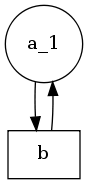
\includegraphics[height=4cm]{img/posti1.png}}
\caption{Esempio di errore nella generazione della rete}\label{fig:err_gen_rete}
\end{figure}
come si può vedere dall'immagine \ref{fig:err_gen_rete} il nome del posto a viene modificato in a\_1 e viene creato un solo
posto.\\
Un altro codice che crea grafi errati è il seguente:
\begin{verbatim}PetriNet n;
Place a,a,a_1;
Transition t;
a_1 -> t -> a -> t;
\end{verbatim}
ovviamente ci si potrebbe aspettare un grafo formato da un arco che vada da un posto chiamato
{\tt a\_1} ad una transizione chiamata {\tt t} e da un cappio tra {\tt t} e {\tt a}.
\begin{figure}[htb]
\centerline{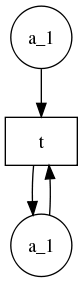
\includegraphics[height=6cm]{img/posti2.png}}
\caption{Rete con due posti con lo stesso nome}\label{fig:err_gen_rete_posti2}
\end{figure}
In realtà il grafo creato è quello mostrato nell'immagine \ref{fig:err_gen_rete_posti2}, un grafo
nel quale compaiono due posti con lo stesso identico nome.


\subsection{Creazione grafo delle marcature}
In PetriNet è possibile creare il grafo delle marcature. Tale procedura è errata e produce 
grafi non corretti. \\
Prendiamo ad esempio il seguente codice:
\begin{verbatim}PetriNet a;
Place x;
Transition t;
x -> t -> x;
M0 = {x};
m={x};
g = a.createCaseGraph(m);
\end{verbatim}
sarebbe corretto attendersi un grafo dei casi {\tt g} a cappio tra un posto relativo alla marcatura 
{\tt \{x\} } con arco chiamato {\tt t}. In realtà il grafo ottenuto sarà un grafo come quello mostrato
in figura \ref{fig:err_grafo_casi_1}.
\begin{figure}[htb]
\centerline{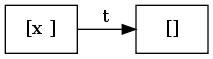
\includegraphics[height=1cm]{img/CG1.jpg}}
\caption{Grafo dei casi errato}\label{fig:err_grafo_casi_1}
\end{figure}
%a.CGtoDot(g,imgGrafoRS,jpg);

\subsubsection{Funzione per creare l'immagine del grafo delle marcature}
Nella sezione precedente abbiamo visto la creazione del grafo delle marcature di una semplice rete. \\
Nel codice non è stata inserita la riga che permette la creazione del file immagine della rete. Per poter
effettuare questa operazione il codice utilizzato è stato: \begin{verbatim}a.CGtoDot(g,imgCG,jpg);\end{verbatim}
La funzione viene chiamata sulla rete base ({\tt a}), passando come parametri il grafo delle marcature ({\tt g}), 
il nome dell'immagine che si vuole creare e l'estensione dello stesso.\\
Essendo le reti viste come oggetti, sarebbe più logico chiamare la funzione direttamente sul grafo delle 
marcature e non sulla rete stessa.

\subsection{Commenti}
Finora in PetriNet non è stata presa in considerazione la possibilità di inserire commenti
nel codice.\\
Dato il carattere descrittivo del linguaggio sarebbe opportuno prevedere questa possibilità
per aiutare il lettore nella comprensione del codice.

\section{Moduli Python}
In questa sezione verranno analizzati i moduli python sviluppati.

\subsection{Stile di programmazione}
All'interno di tutti i moduli sviluppati è stato usato uno stile di programmazione simile a quello
utilizzato per il linguaggio di programmazione Java. Secondo le linee guida ufficiali per Python 
(consigliate dallo stesso Guido Von Rossum a \cite{PYTHCODESTYLE}) lo stile di programmazione 
è leggermente diverso. Una lettura del PEP relativo chiarisce in che modo sarà necessario modificare 
i nomi delle variabili, dei metodi e delle costanti.

\subsection{PetriNet.py}
PetriNet.py contiene le classi utili al funzionamento del parser per il linguaggio.\\
Tutti gli attributi di queste classi hanno nomi comuni ({\tt token}, {\tt nome}, {\tt ...}) pur 
essendo intuitivamente attributi privati. Reimplementando queste classi è stato dunque necessario
cambiarne i nomi e inserire i relativi getters e setters. \\
Le definizioni del metodo {\tt \_\_repr\_\_()} in ogni classe sono scorrette in quanto si cerca di 
utilizzare questo metodo speciale come se fosse il metodo {\tt \_\_str\_\_()}
\footnote{Il metodo {\tt \_\_repr\_\_()} serve a creare una rappresentazione dell'oggetto in modo che
la valutazione della stringa ritornata crei una copia dell'oggetto stesso. Praticamente si averà che 
{\tt eval(repr(x)) == x}.}. \\
Per una trattazione completa degli attributi privati e dei metodi speciali 
si rimanda a \cite{PYTH} o \cite {SUMMERFIELD}.\\
Verranno ora analizzate una per una le classi di questo modulo.

\subsubsection{Obj}
La classe {\tt Obj} è una superclasse dalla quale erediteranno sia le classi {\tt State} e 
{\tt Trans}. Contiene al suo interno siolemente due variabili ({\tt index} e {\tt name}). La 
scelta di inserire il valore indice all'interno degli oggetti verrà rivista nella reimplementazione 
dei moduli in quanto potrebbe creare problemi di inconsistenza.

\subsubsection{State}
State è la classe rappresentante uno stato all'interno del modulo PetriNet.\\
State aggiunge alla classe {\tt Obj} una sola variabile {\tt token} e il metod {\tt \_\_repr\_\_}.
Non si capisce se token sia una variabile booleana che informa se il posto sia pieno o vuoto (si
ricorda che la classe di reti trattate permette posti di capacità 1) oppure se sia un valore intero. 
All'istanziazione dell'oggetto non viene fatto alcun controllo sul valore che assumo le variabili 
passate, di conseguenza {\tt token} potrebbe avere valori negativi.\\
Questa classe accede pubblicamente alle variabili di {\tt Obj} e non dichiara metodi
getter e setter per le sue variabili.

\subsubsection{Trans}
Trans è la classe rappresentante una transizione all'interno del modulo PetriNet.\\
Questa classe non aggiunge nulla alla classe {\tt Obj} ed accede alle variabili della stessa 
come se fossero pubbliche.

\subsubsection{Link}
Link è la classe rappresentante un arco all'interno del modulo PetriNet.\\
Questa classe ha tre variabili {\tt state}, {\tt trans} e {\tt pre}. {\tt state} rappresenta
lo stato relativo all'arco, {\tt trans} la transizione e {\tt pre} il verso dell'arco. \\
La scelta di inserire una variabile booleana che indichi il verso dell'arco è discutibile. 
Questa variabile verrà tolta nella reimplementazione della classe e si controllerà che l'arco
vada da un posto ad una transizione o viceversa durante l'inserimento.

\subsubsection{PetriNet}
PetriNet è la classe rappresentante una rete di Petri all'interno del modulo PetriNet. \\
In questa classse vengono definiti metodi diversi per aggiungere posti, transizioni e link. Nella 
reimplementazione del modulo si è trovato più usabile l'unire queste funzioni all'interno di un semplice
metodo {\tt add} generico che si occupa di inserire l'oggetto passato nel modo corretto.\\
Le strutture dati utilizate per posti, transizioni e archi sono liste; questa scelta implica il fatto
che all'interno del codice si cicli parecchie volte su queste strutture per verificare la presenza 
di un dato oggetto. Se si fosse scelto di utilizzare strutture quali dizionari (forniti nelle librerie 
standard di Python) si sarebbe potuto guadagnare espressività e comprensibilità del codice.
Prendiamop come esempio i seguenti codici che effettuano una ricerca all'interno di una struttura 
dati e stamapano il contenuto se presente.\\
Utilizzando le liste il risultato sarebbe qualcosa di simile:
\begin{verbatim}x = []
[...]
pos = -1
for i in range(len(x)):
    if x[i] == element:
        pos = i
        break
if pos != -1:
    print x[pos] 
else:
    print 'errore'
\end{verbatim}
Mentre, usando i dizionari, il risultato è questo:
\begin{verbatim}x ={}
[...]
if element in x:
# equivalentemente 
# if element in x.keys():
    print x[element]
else:
    print 'errore'
\end{verbatim}
Come si può notare l'utilizzo dei dizionari permette di scrivere codice molto più compatto e comprensibile.
Per questo motivo queste strutture verranno modificate in dizionari.

\subsection{PetriNet\_lex.py}
Questo modulo si occupa della suddivisione in token del codice basandosi sul modulo {\tt lex.py} di
{\tt ply}\footnote{si veda {\tt http://www.dabeaz.com/ply/} per maggiori dettagli su {\tt ply}}. \\
Il modulo è sostanzialmente corretto anche se vengono definiti token non utilizzati nel linguaggio 
(nella fattispecie {\tt in} e {\tt to}).

\subsection{PetriNet\_parser.py}
Questo modulo si occupa della definizione della grammatica formale del linguaggio analizzando la 
sequenza di token trasmessa dal lexer basandosi sul modulo {\tt yacc.py} di {\tt ply}.\\
In questo modulo vengono definite due variabili globali UnionA e UnionB che servono solamente come
appoggio alla funzione unione. La loro visibilità a livello globale non è necessaria.\\
Viene poi definita una classe rete che ricalca sostanzialmente la struttura della classe 
{\tt PetriNet} del modulo {\tt PetriNet.py}; sarebbe stato più chiaro, secondo il mio
punto di vista, utilizzare direttamente la classe {\tt PetriNet.PetriNet}.\\
Dopo la definizione di queste variabili vengono definite le regole per il parsing del linguaggio 
in modo sostanzialmente corretto con quanto finora sviluppato.

%%%%%%%%%%%%%%%%%%%%%%%%%%%%%%%%%%%%%%%%%%%%%%%%%%%

\chapter{Sviluppo di PetriNet}
Nel seguente capitolo verranno mostrate le modifiche apportate al formalismo del linguaggio per ovviare 
ai problemi riportati nel capitolo precedente e le nuove funzionalità dello stesso.

\section{Modifiche vecchie funzionalità di PetriNet}
Nella seguente sezione vengono mostrate le modifiche effettuate alla specifica del linguaggio 
PetriNet con le motivazioni che mi hanno portato ad apportarle. Una trattazione degli aspetti 
modificati può essere trovata nella sezione \ref{sec:linguaggio_petrinet}.

\subsection{Classe di reti trattate}\label{ssect:classe_di_reti_trattate_new}
Uno degli obiettivi del mio stage è stato portare il linguaggio a specificare reti P/T e non più 
solo reti di Petri elementari. È ora possibile in PetriNet definire le capacità dei posti 
e i pesi degli archi (si veda \ref{ssect:nuovi_posti} e \ref{ssect:nuovi_archi} per una 
trattazione migliore dell'argomento) che collegano i vari elementi della rete.

\subsection{Rete Corrente}\label{ssect:rete_corrente_new}
Il concetto di rete corrente è stato eliminato nella reimplementazione di PetriNet. Per 
una migliore comprensibilità del codice è stato scelto di dichiarare sempre la rete sulla quale si 
sta lavorando e non permettere al sistema di inferire automaticamente la rete sulla quale 
si sceglie il focus.\\
È stata scelta questa modalità per ovviare ai problemi riportati nella sezione 
\ref{ssect:Rete_corrente_old}.

\subsection{Nomi dei posti}
Non è più ora possibile definire posti con lo stesso nome all'interno della stessa rete. Nel 
caso ciò si verificasse il programma deve terminare mostrando un errore. In questo modo non sarà 
più possibile avere problemi di ambiguità riguardo ai nomi.\\
Nel caso ora si cercasse di compilare il codice seguente\footnote{Si comprenderà meglio la sintassi della 
dichiarazione dei posti nella sezione \ref{ssect:nuovi_posti}}:
\begin{verbatim}PetriNet x;
Place x::a, x::a;
show_places;
\end{verbatim}
si otterrebbe un output di questo tipo\footnote{Per comodità sono stati eliminati gli output di 
debug che vengono comunque stampati del programma} \footnote{Come si può notare viene usata una 
funzione show\_places, per il suo significato (che può apparire ovvio) si veda il seguito} :
\begin{verbatim}
$ python PetriNet_parser.py -f ~/temp/001.pn 
It seems that an element named a is already in x
\end{verbatim}

\subsection{Creazione del grafo delle marcature}\label{ssect:creazione_grafo_marcature}
Nell'implementazione percedente di PetriNet era possibile creare il grafo delle 
marcature della rete definita. Dato che questo è un aspetto di simulazione mentre 
l'obiettivo di questo sistema è quello di fornire un linguaggio di specifica per la rete,
dato che l'implementazione della creazione di grafi delle marcature era errata e quindi
sarebbe stato necessario riscrivere anche questo pezzo di codice è stato deciso di 
eliminare queste funzionalità.\\
La decisione presa non limita le possibilità fornite dall'utilizzo di PetriNet in quanto, come
si vedrà in seguito, è stata aggiunta la possibilità di esportare le reti in un formato adatto a 
software di simulazione\footnote{Vedi programma pipe a http://pipe2.sourceforge.net/} che creano 
grafi delle marcature in modo corretto.

\subsection{Commenti}\label{ssect:new_commenti}
Nella nuova implementazione di PetriNet è stata aggiunta la possibilità di inserire commenti all'interno del 
codice. Volendo mantenere uno stile {\tt c}-like (decisione presa precendetemente al mio stage) si è optato 
per la possibilità di inserire commenti monoriga preceduti dai caratteri {\tt //}. Il seguente esempio mostra 
dei commenti innestati nel codice:
\begin{verbatim}PetriNet net;
Place net::a, net::b; // Commento a fine riga
// Commento che prende tutta la riga
Transition net::x, net::y;
\end{verbatim}

\subsection{Marcatura iniziale}
\begin{figure}[htb]
\centerline{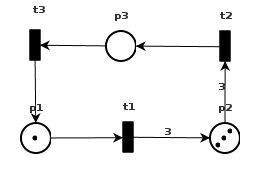
\includegraphics[width=7cm]{img/test_marcature.png}}
\caption{Esempio di semplice rete con marche}\label{fig:test_marcature.png}
\end{figure}
Il modo di definire una marcatura in PetriNet è stato modificato totalmente per poter essere utilizzabile con reti che hanno posti con capacità maggiore di 1.
Il modo migliore per poter spiegare questo nuovo metodo è mostrando un esempio.
\begin{verbatim}PetriNet net;
Place net{p1, p2(5), p3};
Transition net{t1, t2, t3};

net{p1 -> t1 ->(3) p2 ->(3) t2 -> p3 -> t3 -> p1};

net{p1=1, p2=3};
\end{verbatim}

Nell'esempio appena scritto viene create una rete contenente 3 posti ({\tt p2] con capacità 5} e 3 transizione. 
Successivamente viene definito il flusso della rete descrivendo una rete circolare e dopodiché viene istanziata la marcatura iniziale della rete con il codice {\tt net{p1=1, p2=3}}
 che inserisce una marca in {\tt p1} e 3 marche in {\tt p2}. Una rappresentazione di questa rete è mostrata in figura \ref{fig:test_marcature.png}.\\
Ovviamente, nel caso si cercasse di inserire una quantità di marche maggiore alla capacità di un posto, il sistema fornirà un errore.

\section{Nuove funzionalità di PetriNet}
Nella seguente sezione vengono mostrate le innovazioni apportate al linguaggio PetriNet.

\subsection{Direttive al parser}\label{subsec:direttive_al_parser}
Durante la progettazione del sistema PetriNet ci si è accorti che non
necessariamente tutte le reti definite debbano sottostare ad assunti
uguali. Un esempio abbastanza banale è il fatto che alcune reti
potrebbero richiedere posti con capacità 1 come default mentre alcune
potrebbero assumere una capacità illimitata come comportamento
standard. \\
Per far fronte a questo problema è stato deciso di inserire la
possibilità di modificare il comportamento del sistema inserendo
direttamente nel codice delle direttive\footnote{Chiamate per
  chiarezza direttive al parser in quanto sono valori che vengono
  considerati da questa componente del sistema}.\\
Per poter passare una direttiva al parser lo schema generale è
banalmente il
seguente: \\
{\tt \# nome\_parametro=valore\_parametro;} \footnote{\'E stata
  scelta questa sintassi in quanto simile alle direttive al
  preprocessore del linguaggio c e quindi è possibile utilizzare i
  sintax highlighting di alcuni ambienti di sviluppo} \\
Attualmente i valori gestiti da PetriNet sono
\emph{default\_place\_capacity}, \emph{union\_type} e
\emph{union\_add\_prefix}. Per una trattazione dei due parametri
relativi all'unione di reti si rimanda alla sezione dedicata
\ref{subsect:unione_di_reti} mentre la prima verrà spiegata ora. \\
Il parametro \emph{default\_place\_capacity} influisce sulla
dichiarazione di posti nel codice. Come precedentemente accennato
potrebbe essere necessario avere reti con capacità di default diversa,
grazie a questo parametro è possibile modificare questo comportament
assegnandovi un numero positivo oppure il valore unlimited. \\
Nel caso si dichiari \emph{default\_place\_capacity} come unlimited il
sistema assegnerà ai posti una capacità di default concettualmente
illimitata ma, in realtà, essa sarà comunque limitata al numero intero
massimo gestibile dalla versione di python sottostante al sistema.

\subsection{Array di reti}
Nella specifica di reti è possibile dover realizzare modelli con la stessa struttura base che 
definiscono componenti del sistema che si comportano nello stesso modo. Finora per poter modellare 
una situazione simile era necessario creare una componente alla volta ripetendo svariate volte 
le stesse righe di codice. Provando a pensare alla modellazione di un numero elevato di processi è 
facile comprendere come il codice diventasse di una lunghezza difficilmente contenibile. \\
Per ovviare a questo problema è stato deciso di dare la possibilità di creare array monodimensionali 
di reti. In questo modo è possibile descrivere solamente una volta il comportamento e applicarlo ad 
ogni componente interessata.

\subsubsection{Dichiarazione}
{\tt PetriNet} \emph{nomereti}{\tt[}\emph{cardinalità}{\tt], \emph{\dots};}\\
\\
Per poter definire array di reti, come prevedibile, sarà necessario dare a priori una grandezza 
dell'array stesso ponendo la cardinalità all'interno di due parentesi quadre poste successivamente al nome 
dell'array, come nella maggior parte dei linguaggi di programmazione\footnote{L'indice ammissibile per una 
rete dichiarata di cardinalità n andrà da 0 a n-1}.\\
Per esempio:
\begin{verbatim}PetriNet philosophers[5];
\end{verbatim}
creerà 5 reti che potrebbero successivamente venire modellate come nel classico esempio dei filosofi.\\
È permessa l'istanziazione di array sulla stessa riga, di conseguenza il seguente codice:
\begin{verbatim}PetriNet philosophers[5], fork[5];
\end{verbatim}
è corretto secondo le specifiche di PetriNet.\\
È inoltre possibile mischiare le dichiarazioni di array di reti e di reti "normali". Il seguente codice quindi
è da considerarsi corretto:
\begin{verbatim}PetriNet philosophers[5], monitor, fork[5];
\end{verbatim}
Si può fin da ora notare come ci sia già un marcato guadagno in lunghezza e chiarezza del codice derivante 
da questa nuova funzionalità dovuto anche alla sola dichiarazione di reti (precedentemente sarebbero dovute 
venir dichiarate una per una tutte le reti).

\subsubsection{Modellazione}
È possibile, come precedentemente accennato, modellare il comportamento di tutte le reti appartenenti ad un 
array in modo che siano uguali. Il seguente codice\footnote{Le linee di codice sono state spezzate su più 
righe. Il codice del flusso di transizioni, per funzionare, deve essere scritto su una riga sola} \footnote{
Vengono in questo momento tagliate parti di codice (dichiarazione di posti e di transizioni, altri comandi) in
quanto non ancora trattati}:
\begin{verbatim}PetriNet philosophers[5];
[...]
philosophers{think -> get_ready -> ready -> get_left 
	     -> got_left -> get_right -> got_right -> 
	      eat -> release -> think};
[...]
\end{verbatim}
crea la struttura base di ogni rete di philosophers in modo che ogni componente si comporti esattamente nello
stesso modo.\\
È ragionevole pensare che in alcuni casi qualche componente abbia un comportamento particolare  pur basandosi 
sullo stesso schema delle sue reti "simili". Per questo è possibile aggiungere posti, transizioni e archi di 
flusso ad ogni singola rete appartentente ad un array.\\
Il seguente codice:
\begin{verbatim}PetriNet philosophers[5];
[...]
philosophers{think -> get_ready -> ready -> get_left 
	     -> got_left -> get_right -> got_right -> 
	      eat -> release -> think};
[...]
philosophers[0]{get_ready -> times};
[...]
\end{verbatim}
aggiunge arco alla prima rete dell'array {\tt philosophers} che va da una (possibile) transizione {\tt get\_ready}
ad un (possibile) posto {\tt times} che potrebbe funzionare come contatore per questo componente.

\subsection{Dichiarazione di posti}\label{ssect:nuovi_posti}
Nella nuova implementazione di PetriNet è possibile definire posti in diverse modalità.\\

\begin{itemize}

\item Il primo metodo è dichiarando un posto come ``attributo'' della rete nel seguente modo:
\begin{verbatim}PetriNet x;
Place x::a;
\end{verbatim}
dopo aver eseguito tale codice si avrà una rete {\tt x} contentente un posto {\tt a}.
È ovviamente possibile dichiarare più posti in successione sulla stessa riga separati da 
virgole. Il codice seguente è corretto secondo la nuova specifica di PetriNet:
\begin{verbatim}PetriNet x;
Place x::a, x::b;
\end{verbatim}
È anche possibile dichiarare posti appartenti a reti diverse sulla stessa riga nel seguente modo:
\begin{verbatim}PetriNet x, y;
Place x::a, y::a, x::b, y::c;
\end{verbatim}

\item Il secondo metodo è dichiarando una lista di posti appartenenti ad una rete nel seguente modo:
\begin{verbatim}PetriNet x;
Place x{a, b, c};
\end{verbatim}
che creerà una rete contenente i posti {\tt a}, {\tt b} e {\tt c}.

\item Esiste una terza possibilità, della quale si scoraggia l'utilizzo, per inserire posti in una rete.
Questa modalità sfrutta la capacità del sistema di fornire le funzioni dei moduli python al linguaggio PetriNet
(verrà mostrato in seguito questo aspetto). Di conseguenza è possibile definire posti ``generici'' slegati da 
ogni rete e poi andare ad aggiungerli alle reti che ci interessano. Il seguente codice potrà aiutare a chiarire
le idee a riguardo:
\begin{verbatim}PetriNet x;
Place y;
x::add(y);
\end{verbatim}
come si può notare viene chiamata la funzione {\tt add} sulla rete {\tt x} passando come parametro {\tt y}.
Andando a guardare il codice python dell'implementazione delle reti di Petri si può vedere come la classe 
{\tt PetriNet} (che definisce ovviamente il concetto di rete di Petri) ha al suo interno la funzione {\tt add}
alla quale è possibile passare un qualsiasi elemento.\\
Questo metodo è scoraggiato in quanto poco funzionale e complica inutilmente il codice.
\end{itemize}

\subsubsection{Posti con pesi}
Come detto nella sezione \ref{ssect:classe_di_reti_trattate_new} il sistema è stato portato a definire 
classi P/T e quindi deve essere possibile definire una capacità per i posti. Ciò è possibile inserendo, dopo il 
nome del posto, un numero intero e positivo racchiuso all'interno di parentesi tonde. Per esempio
\begin{verbatim}PetriNet x;
Place x::p1(3);
Place x{p2(5), p3};
\end{verbatim}
sono dichiarazioni valide. Mentre:
\begin{verbatim}PetriNet x;
Place x::p1(-6);
Place x{a(0)};
\end{verbatim}
non sono dichiarazioni valide.\\
Nel caso non venga dichiarata alcuna capacità il sistema assume il
valore di default selezionato nelle direttive al parser.

\subsubsection{Array di posti}
Come per le reti, è possibile creare array di posti in modo da poter rendere più compatto il codice.
Il seguente esempio contiene dichiarazioni di posti ammissibili:
\begin{verbatim}PetriNet foo[5];
Place foo{ bar[3], baz}, foo[0]{ tar(8)};
Place foo::zip(7), foo[1]::apt(3);
\end{verbatim}
come si può notare le combinazioni possibili per poter dichiarare posti in una rete sono molto varie
e sono abbastanza comprensibili.\\
È stato scelto nell'implementazione che tutti i posti appartenenti ad un array debbano avere la stessa capacità 
in quanto un array di posti rappresente una collezione di posti uguali e sarebbe poco logico averne con capacità 
diverse.

\subsection{Transizioni}
Equivalentemente ai posti è possibile dichiarare transizioni in 3 modi diversi:

\begin{itemize}

\item Dichiarando una transizione come ``attributo'' di una rete nel seguente modo:
\begin{verbatim}PetriNet x, y;
Transition x::a, x::b, y::b, x::c;
\end{verbatim}

\item Dichiarando una lista di transizioni appartenenti ad una rete:
\begin{verbatim}PetriNet x;
Transition x{ a,b,c};
\end{verbatim}

\item Aggiungendo una transizione ad una rete tramite il metodo add:
\begin{verbatim}PetriNet x;
Transition a;
x::add(a);
\end{verbatim}
come per i posti l'utilizzo di questo metodo di inserimento è fortemente scoraggiato.

\end{itemize}

\subsubsection{Array di transizioni}
Anche per le transizioni è possibile definire array per avere transizioni logicamente simili raggruppate
sotto lo stesso nome.\\
\\
Le seguenti dichiarazioni di transizioni sono tutte corrette:
\begin{verbatim}PetriNet foo[5];
Transition foo{ bar[3], baz}, foo[0]{ tar}, foo::zip, foo[1]::apt;
\end{verbatim}


\subsection{Definizione flussi}\label{ssect:nuovi_archi}
La sintatssi per la definizione di flussi in PetriNet è stata rivista completamente ed è stata 
reimplementata ispirandosi leggermente al linguaggio di specifica FSP\footnote{ Si veda 
http://www.doc.ic.ac.uk/~jnm/LTSdocumention/FSP-notation.html per maggiori dettagli}.\\
Per poter definire un flusso all'interno di una rete sarà necessario ora specificare su quale rete si stia 
lavorando in questo momento e successivamente raccogliere tra parentesi graffe una lista di posti e transizioni
collegati tra di loro dai caratteri {\tt ->}. In questo modo si specificheranno percorsi all'interno della 
rete e il comportamente di ogni componenete sarà facilmente intuibile.
È possibile definire più flussi in due modi:
\begin{itemize}

\item ``Aprendo'' due volte la rete ed inserendo un percorso nel seguente modo:
\begin{verbatim}PetriNet net;
Place net{a,b,c};
Transition net{x,y};
net{ a -> x -> c};
net{ a -> y -> b};
\end{verbatim}

\item Definendo un percorso alternativo con l'inserimento del simbolo di OR {\tt |}:
\begin{verbatim}PetriNet net;
Place net{a,b,c};
Transition net{x,y};
net{ a -> x -> c | a -> y -> b};
\end{verbatim}
\end{itemize}

In entrambi i casi il risultato sarà quello riportato in figura \ref{fig:flussi1.png}.
\begin{figure}[htb]
\centerline{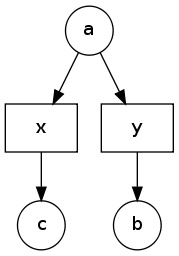
\includegraphics[height=4cm]{img/flussi1.png}}
\caption{Rete semplice generata con doppio inserimento di flusso}\label{fig:flussi1.png}
\end{figure}

Per ora non è ancora possibile collegare array di posti e transizioni ma solo elementi di questi array.
Il codice 
\begin{verbatim}PetriNet net;
Place net{x[2], z};
Transition net{y};
net{ x -> y -> z};
\end{verbatim}
di conseguenza non ha alcun risultato ma sarà necessario collegare ogni elemento di {\tt x} alla transizione
nel seguente modo:
\begin{verbatim}PetriNet net;
Place net{x[2], z};
Transition net{y};
net{ x[0] -> y -> z | x[1] -> y};
\end{verbatim}
per ottenere quanto mostrato in figura \ref{fig:flussi2.png}.

\begin{figure}[htb]
\centerline{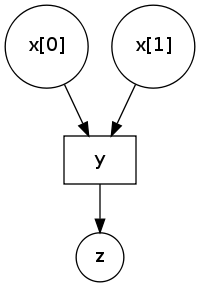
\includegraphics[height=4cm]{img/flussi2.png}}
\caption{Rete semplice generata con doppio inserimento di flusso}\label{fig:flussi2.png}
\end{figure}

\subsubsection{Archi pesati}
Come detto nella sezione \ref{ssect:classe_di_reti_trattate_new} il sistema è stato portato a definire 
classi P/T e quindi deve essere possibile definire archi con pesi diversi da 1. Ciò è possibile inserendo, dopo
i caratteri {\tt ->} un numero intero positivo racchiuso all'interno di parentesi tonde. Per esempio la seguente
porzione di codice:
\begin{verbatim}PetriNet net;
Place net{ buffer(8)};
Transition net{consuma_token, consuma_2_token};
net{ buffer -> consuma_token};
net{ buffer ->(2) consuma_2_token};
\end{verbatim}
crea la rete presentata in figura \ref{fig:flussi3.png} nella quale si vede che l'arco tra il posto {\tt buffer}
(di capacità 8) e la transizione {\tt consuma\_2\_token} ha peso 2.

\begin{figure}[htb]
\centerline{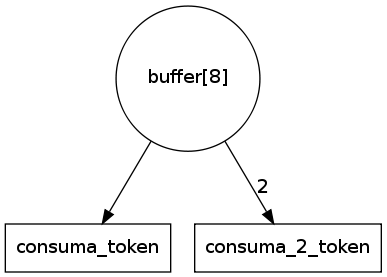
\includegraphics[height=5cm]{img/flussi3.png}}
\caption{Rete con archi pesati}\label{fig:flussi3.png}
\end{figure}

\subsection{Unione di reti}\label{subsect:unione_di_reti}
Per migliorare la comprensibilità di un codice scritto in linguaggio PetriNet è possibile creare delle reti che descrivano il comportamento di una componente per poi unire tutte queste sottoreti in una rete di Petri.\\
L'unione di reti era presente anche nella versione precedente del linguaggio PetriNet ma presentava qualche problema sulla gestione della sovrapposizione di posti e transizioni.\\
È possibile comporre \emph{n} reti sia per sovrapposizione di posti sia per sovrapposizione di transizioni e lo schema generale dell'unione di \emph{n} reti è il seguente:\\

\emph{rete}  = emph{\tt(}\emph{lista-reti}{\tt)} on
{\tt[}\emph{lista-elementi-unione-1},\emph{lista-elementi-unione-2},
\dots \emph{lista-elementi-unione-n},{\tt]};\\

dove:\\

\emph{lista-reti} = \emph{nome-rete-1} | \emph{nome-rete-2} | \dots
\emph{nome-rete-n} \\

\emph{lista-elementi-unione} = \emph{elemento-rete-1} =
\emph{elemento-rete-2} = \dots = \emph{elemento-rete-n} as
\emph{nuovo-nome} \\

\'E  possibile lasciare \emph{lista-elementi-unione} vuota. \\
Il comportamento dell'operazione di unione è diverso a seconda delle
direttive che vengono passate al parser. Le direttive che riguardano
l'unione sono due ed esattamente quelle chiamate \emph{union\_type} e
\emph{union\_add\_prefix}.\\
La direttiva \emph{union\_type} ha due valori possibili:
\begin{description}
\item{{\bf only\_when\_equal}}: in questo caso sarà possibile
  sovrapporre posti solamente nel caso in cui abbiano marcature e
  capacità uguali [comportamento di default]
\item{{\bf override}}: in questo caso sarà possibile sovrapporre i
  posti sempre e gli elementi avranno la capacità e la marcatura del
  posto appartente alla prima rete della lista.
\end{description}
La direttiva \emph{union\_add\_prefix} è un valore booleano (valori
"True" e "False") che permette di decidere se durante l'unione i posti
che non vengono uniti esplicitamente nella
\emph{lista-elementi-unione} debba venir aggiunto come prefisso il
nome della rete alla quale appartengono o meno. Nel caso questo valore
venisse impostato a {\tt False} e nel caso in due reti esistano
elementi con lo stesso nome essi verranno trattati come uno solo
nell'unione e, di conseguenza, verranno collegati tutti gli elementi
delle reti unite.\\
\'E comunque sconsigliato creare reti partendo da modelli nei quali
esistano elementi con lo stesso nome che non verranno uniti.\\
La \emph{lista-elementi-unione} per ora deve necessariamente essere
un'espressione di {\tt n} elementi dove {\tt n} è il numero di reti
che partecipano alla procedura di unione. \'E molto facile notare che
non necessariamente tutte le reti prendano parte con dei propri
elementi ad una sovrapposizione, in questo caso, nell'elencare gli
elementi, sarà sufficiente inserire la parola "null" nella posizione
della rete che non partecipa all'unione.

\subsubsection{Esempi}
Per capire meglio il funzionamento dell'unione portiamo ora alcuni semplici
esempi facilmente comprendibili. Per esempi più complessi si rimanda al capitolo
\ref{cap:esempi}.
\subsubsection{Esempio 1}
\begin{figure}[htb]
\centerline{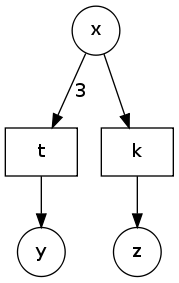
\includegraphics[height=5cm]{img/unione_001.png}}
\caption{Risultato esempio 1}\label{fig:unione_001.png}
\end{figure}
Unione di due reti con posti con lo stesso nome e senza direttiva di aggiunta
di prefisso.\\
{\bf Codice}
\begin{verbatim}
PetriNet a,b;
Place a{x,y}, b{x,z};
Transition a::t, b::k;

a{x ->(3) t -> y};
b{x -> k -> z};

sys = (a | b) on [];
\end{verbatim}


\subsubsection{Esempio 2}
\begin{figure}[htb]
\centerline{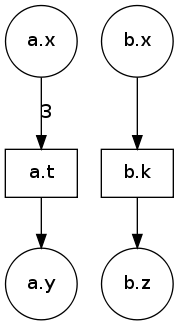
\includegraphics[height=5cm]{img/unione_002.png}}
\caption{Risultato esempio 2}\label{fig:unione_002.png}
\end{figure}
Unione di due reti con posti con lo stesso nome e con direttiva di aggiunta
di prefisso.\\
{\bf Codice}
\begin{verbatim}
PetriNet a,b;
Place a{x,y}, b{x,z};
Transition a::t, b::k;

a{x ->(3) t -> y};
b{x -> k -> z};

#union_add_prefix=True;
sys = (a | b) on [];
\end{verbatim}


\subsubsection{Esempio 3}
\begin{figure}[htb]
\centerline{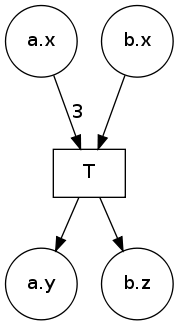
\includegraphics[height=5cm]{img/unione_003.png}}
\caption{Risultato esempio 3}\label{fig:unione_003.png}
\end{figure}
Unione di due reti con posti con lo stesso nome, con direttiva di aggiunta
di prefisso e con dichiarazione di unione delle transizioni.\\
{\bf Codice}
\begin{verbatim}
PetriNet a,b;
Place a{x,y}, b{x,z};
Transition a::t, b::k;

a{x ->(3) t -> y};
b{x -> k -> z};

#union_add_prefix=True;
sys = (a | b) on [t = k as T];
\end{verbatim}


\subsubsection{Esempio 4}
In questo caso si cerca di sovrapporre due elementi con capacità diverse.\\
{\bf Codice}
\begin{verbatim}
PetriNet a,b;
Place a{x(75),y}, b{x,z};
Transition a::t, b::k;

a{x ->(3) t -> y};
b{x -> k -> z};

#union_add_prefix=False;
#union_type=only_when_equal;
sys = (a | b) on [t = k as T, x = x as X];
\end{verbatim}
{\bf Risultato esempio 4}\\
Errore in quanto x della rete a e x della rete b hanno capacità diverse


\subsubsection{Esempio 5}
\begin{figure}[htb]
\centerline{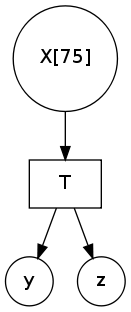
\includegraphics[height=5cm]{img/unione_004.png}}
\caption{Risultato esempio 5}\label{fig:unione_004.png}
\end{figure}
In questo caso si cerca di sovrapporre due elementi con capacità diverse
dichiarando correttamente la direttiva union\_type.\\
{\bf Codice}
\begin{verbatim}
PetriNet a,b;
Place a{x(75),y}, b{x,z};
Transition a::t, b::k;

a{x ->(3) t -> y};
b{x -> k -> z};

#union_add_prefix=False;
#union_type=override;
sys = (a | b) on [t = k as T, x = x as X];
\end{verbatim}

\subsubsection{Esempio 6}

In questo esempio vengono sovrapposte tre reti su elementi diversi.\\
{\bf Codice}
\begin{verbatim}
PetriNet a,b,c;
Place a{x,y}, b{x,z}, c{u,s};
Transition a::t, b::k, c::r;

a{x ->(3) t -> y};
b{x -> k -> z};
c{u -> r ->(2) s};

#union_add_prefix=False;
sys = (a | b | c) on [t = k = null as T, null = z = s as Z];
\end{verbatim}
\begin{figure}[htb]
\centerline{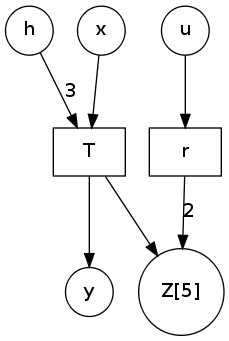
\includegraphics[height=7cm]{img/unione_006.png}}
\caption{Risultato esempio 6}\label{fig:unione_006.png}
\end{figure}
\newpage


\subsection{Ciclo for}
Uno degli obiettivi principali del mio lavoro svolto su PetriNet era
quello di implementare una funzione simile ai cicli for presenti in
quasi la totalità dei linguaggi di programmazione. \\
Questa funzionalità è utile perché permette di diminuire lo sforzo
nella scrittura del codice, diminuisce la lunghezza dello stesso e
rende concettualmente più chiaro il flusso delle istruzioni.\\
La sintassi dei cicli simile a quella classica della maggior parte dei
linguaggi di programmazione che può essere schematizzata nel seguente
modo:
\begin{verbatim}
for(condizioni_iniziali;condizioni_finali;incrementi){
istruzione_1;
istruzione_2;
...
istruzione_n;
}
\end{verbatim}
dove: \emph{condizioni\_iniziali} serve ad inizializzare le variabili
utilizzate come parametri all'interno del codice,
\emph{condizioni\_finali} serve ad impostare le condizioni di uscita
dal ciclo e \emph{incrementi} sono le istruzioni da eseguire ogni volta
che un ciclo termina. \\
Ogni condizione può essere multipla, in questo caso ogni istruzione
deve essere separata dalle altre utilizzando una virgola. \\
Per ora il ciclo termina quando tutte le condizioni finali sono verificate. 
Non è stata per implementata la possibilità di utilizzare operatori logici 
{\tt or} e {\tt and} in quanto PetriNet è pensato come linguaggio descrittivo
e non come linguaggio di programmazione. Sarà comunque possibile in futuro
migliorare questo aspetto.\\

\subsubsection{Espressioni matematiche}
È possibile, all'interno di un blocco for, utilizzare le variabili dichiarate 
come indici di array di posti, transizioni o reti. È stato inoltre sviluppato
un rudimentale sistema che permette di gestire correttamente i calcoli 
base che vedono coinvolte le variabili. Ciò vuol dire che il seguente estratto 
di codice è corretto:
\begin{verbatim}
for(i=0;i<10;i+=1){
net{ p[i] -> t[i] -> p[i+1]};
}
\end{verbatim}
In questo caso l'espressione \emph{i+1} viene correttamente interpretata dal 
sistema PetriNet. \\
In PetriNet sono gestiti i seguenti operandi tra variabili e valori interi:
\begin{description}
\item[+] per la somma 
\item[-] per la sottrazione
\item[*] per la moltiplicazione
\item[/] per la divisione 
\item[\%] per calcolare il modulo di due valori
\end{description}
Non è possibile raggruppare elementi in parentesi tonde per gestire la precedenza
delle operazioni in quanto non ci si è soffermati troppo sulla gestione
delle espressioni matematiche. L'ordine in cui le operazioni vengono effettuate 
è lo stesso in cui sono state presentate nel precedente elenco.\\
\\
Anche nelle condizioni di inizio, fine e incremento del ciclo sono presenti
delle espressioni matematiche. In queste espressioni è possibile utilizzare 
qualsiasi costrutto matematico conosciuto dalla versione Python utilizzata
\footnote{Questo vuol dire che il costrutto {\tt ++} non è utilizzabile e che 
il codice {\tt x++} dovrà essere sostituito dal codice {\tt x+=1}.}.

\subsubsection{Cicli innestati}
È possibile utilizzare i cicli for in modo annidato. In questo caso tutte le 
variabili dichiarate nel ciclo esterno saranno utilizzabili anche nel ciclo 
interno.\\
Il seguente codice di conseguenza è corretto:
\begin{verbatim}
for(i=0; i<5; i+=1){
  for(j=0; j<i; j+=1){
    net{p[i] -> t[j] -> p[i+1]}; 
  }
}
\end{verbatim}

\subsubsection{Limitazioni sui pesi degli archi}
Per ora non è possibile utilizzare le variabili dei cicli come 
pesi per i posti degli archi.

% TODO : scrivere sezione


% Quando la lista di elementi è presente, invece, nella nuova rete verrà inserito un posto o transizione con il nome del primo elemento nel caso i due nomi siano diversi.\\
% Nel caso ci siano posti con nomi in conflitto appartenenti alle due reti e non sovrapposti nell'unione delle reti il loro nome verrà modificato aggiungendo come prefisso il nome della rete alla quale appartengono\footnote{Nel caso in cui il nome di tale elemento sia ancora in conflitto all'interno delle reti, il prefisso verrà aggiunto ricorsivamente}.\\
% È possibile, per ora, unire solo due reti alla volta.

%%%%%%%%%%%%%%%%%%%%%%%%%%%%%%%%%%%%%%%%%%%%%%%%%%%%%%%%%%%%%%%%%%

\section{Moduli Python}
All'interno di questa sezione verranno mostrate le modifiche apportate ai moduli Python sviluppati
per il linguaggio PetriNet.

\subsection{Stile di programmazione}
Durante la riscrittura del codice si è cercato di portare lo stile di programmazione il più vicino possibile 
a quanto consigliato da Guido Von Rossum a \cite{PYTHCODESTYLE}. Il vecchio codice non faceva utilizzo di 
list comprehension che sono molto utili per scrivere codice compatto, ove possibile si è cercato di utilizzare
questa funzionalità del linguaggio.

\subsection{PetriNet.py}

\begin{figure}[htb]
\centerline{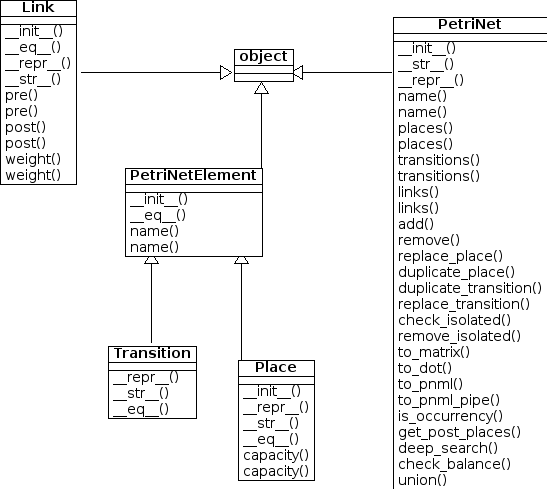
\includegraphics[height=8cm]{img/uml_pyth.png}}
\caption{Diagramma UML delle classi Python sviluppate}\label{fig:uml_pyth.png}
\end{figure}

I nomi degli attributi di ogni classe del modulo PetriNet.py sono stati modificati rendendoli attributi privati
e creando i relativi metodi getter e setter. \\
Per quasi ogni classe sono stati creati i metodi speciali {\tt \_\_repr()\_\_}, {\tt \_\_str()\_\_} e 
{\tt \_\_eq\_\_()} corretti. È possibile vedere uno schema UML del sistema sviluppato nell'immagine \ref{fig:uml_pyth.png}.\\
Verranno ora analizzate le classi di questo modulo.

\subsubsection{PetriNetElement}
La classe PetriNetElement prende il posto della classe Obj del sistema sviluppato precedentemente. Il cambio
di nome è stato effettuato per aumentare la comprensibilità del codice in quanto Obj non dava alcuna informazione
sul tipo di dato ed era confondibile con la classe {\tt object} di Python.
In questa classe viene definito un attributo di nome name che sta ad indicare il nome dell'oggetto e i relativi
getter e setter.

\subsubsection{Place}
Place è la classe rappresentante un posto all'interno del modulo PetriNet. L'unico attributo aggiunto da questa classe alla classe PetriNetElement (dalla quale deriva) è capacity che sta ad indicare, appunto, la capacità del posto. Vengono definiti i metodi speciali {\tt \_\_repr()\_\_}, {\tt \_\_str()\_\_} e {\tt \_\_eq\_\_()} e il gettere e il setter per l'attributo capacity.

\subsubsection{Transition}
Transition è la classe rappresentante una transizione all'interno del modulo PetriNet. Deriva dalla classe PetriNetElement e ridefinisce i metodi {\tt \_\_repr()\_\_} e {\tt \_\_str()\_\_} senza aggiungere alcun altro attributo.

\subsubsection{Link}
La classe Link rappresenta un arco all'interno del modulo PetriNet. Nel reimplementare la classe è stato eliminato l'attributo pre che indicava il verso dell'arco. Ora questa classe contiene due soli attributi, {\tt pre} che indica lo stato o transizione dal quale l'arco parte e {\tt post} che indica a quale stato o transizione l'arco arriva.\\
Altra modifica apportata è stata l'aggiunta di un attributo {\tt weight} che indica il peso dell'arco, nell'inizializzazione dell'oggetto questo valore assume come default 1 e non è possibile inserire valori negativi o 0.\\
Sono stati definiti anche tutti i metodi getters e setters per ogni attributo della classe.

\subsubsection{PetriNet}
PetriNet è la classe rappresentante una rete di Petri all'interno del modulo PetriNet.\\
Questa classe ha quattro attributi: {\tt name}, {\tt places}, {\tt transitions} e {\tt links}. Il primo è il nome della rete mentre gli altri sono liste contenenti rispettivamente posti, transizioni e archi.\\
In questa classe sono stati raggruppati tutti i metodi per inserire oggetti all'interno della rete in un solo metodo chiamato per l'appunto {\tt add} che si occupa di capire il tipo di oggetto passatogli e di aggiungerlo alla struttura dati adeguata. Sono stati inoltre implementati metodi per la rimozione dei posti e delle transizioni e per il rimpiazzamento di questi elementi.\\
È stata inoltre inserita la possibilità di esportare una rete in formato {\tt pnml}. Come si può notare dando una rapida lettura al codice sono stati implementati due diversi metodi che permettono di esportare in questo formato. Questa scelta è dovuta al fatto che il programma {\tt pipe} non rispetta completamente lo standard {\tt pnml} e, ad esempio, usa l'attributo {\tt value} invece che {\tt text} per indicare alcuni valori. Purtroppo, non avendo ancora trovato un algoritmo di posizionamento adatto per le reti di Petri tutti gli elementi esportati in {\tt pnml} saranno posizionati automaticamente dal metodo in posizione {\tt (0, 0)} e sarà necessario spostarli manualmente per creare una vista migliore della rete. \\
In questa classe sono stati rimossi i metodi per la creazione del grafo delle marcature per le motivazioni spiegate nella sezione \ref{ssect:creazione_grafo_marcature}.

\subsection{PetriNet\_lex.py}
Come precedentemente detto questo modulo si occupa della suddivisione in token del codice basandosi sul modulo {\tt lex.py} di {\tt ply}.\\
Nella reimplementazione sono stati eliminati i token inutilizzati precedentemente e sono state inserite seguenti regole:
\begin{description}

\item[{\tt '|'}] per consentire di riconoscere l'{\tt or} nella descrizione di flussi1

\item[{\tt 'COMMENT'}] per riconoscere i commenti all'interno del codice (si veda la sezione \ref{ssect:new_commenti})

\item[{\tt 'ARRAY\_ID'}] per riconoscere un identificatore di array

\item[{\tt 'DDOT'}] per riconoscere il doppio due punti ({\tt ::}) per permettere di accedere a funzioni di una rete in stile ({\tt C++})

\item[{\tt 'STRING'}] per riconoscere stringhe (questa regola è diversa dalla regola ID in quanto in una stringa possono essere presenti caratteri non accettabili per un ID)

\end{description}

Sono inoltre state inseriti i seguenti token utili per il debug:
\begin{description}

\item[{\tt 'show\_places'}] che permetterà di stampare a video i posti dichiarati in un certo momento

\item[{\tt 'show\_transitions'}] che permetterà di stampare a video le transizioni dichiarate in un certo momento

\item[{\tt 'show\_nets'}] che permetterà di stampare a video le reti dichiarate in un certo momento

\item[{\tt 'show\_links'}] che permetterà di stampare a video gli archi dichiarati in un certo momento

\end{description}

Sono stati anche eliminati e seguenti token presenti precedentemente:

\begin{description}

\item[{\tt 'toDot'}] in quanto, come si vedrà successivamente è stata implementata una funzione in  {\tt PetriNet\_parser.py} che è in grado di richiamare ogni funzione della classe {\tt PetriNet} senza dover dichiarare token dedicati

\item[{\tt 'isOccurrency'}] per lo stesso motivo del token {\tt toDot}

\item[{\tt 'matrix'}] per lo stesso motivo del token {\tt toDot}

\item[{\tt 'createCaseGraph'}] in quanto non più presente questa funzionalità

\item[{\tt 'CGtoDot'}] in quanto non più presente la funzionalità di creare grafi delle marcature

\item[{\tt 'WorkOn'}] in quanto non più presente il concetto di rete corrente (si veda sezione \ref{ssect:rete_corrente_new})

\item[{\tt 'ADD'}] per lo stesso motivo del token {\tt toDot}

\item[{\tt 'for'}] in quanto inutilizzato anche precedentemente e non ancora implementati i cicli

\item[{\tt 'to'}] in quanto inutilizzato

\item[{\tt 'in'}] in quanto inutilizzato

\end{description}


\subsection{PetriNet\_parser.py}
\begin{verbatim}
$ ./PetriNet_parser.py --help
Usage: PetriNet_parser.py [-f INPUT_FILE] [-i] 

Options:
  -h, --help            show this help message and exit
  -f INPUT_FILE, --file=INPUT_FILE
                        File su cui richiamare il parser
  -i, --interactive     Esegue il parser in modo interattivo 
                        (in questo caso il file passato non 
                        viene preso in considerazione)
\end{verbatim}
Questo modulo si occupa della definizione della grammatica formale del linguaggio analizzando la sequenza di token trasmessa del lexer.\\
In questo modulo sono state eliminate le variabili globali inutili precedentemente presenti ({\tt UnionA} e {\tt UnionB}).\\
Essendo stato eliminato il concetto di rete corrente è stata eliminata la variabile {\tt actualNet} e la definizione della classe {\tt rete}. Il dizionario {\tt net} è poi stato rinominato in {\tt nets} e sono stati creati dei dizionari chiamati {\tt places}, {\tt transitions} e {\tt links} che contengono rispettivamente i posti, le transizioni e gli archi dichiarati non appartenenti ad alcuna rete\footnote{Esisite attualmente, in PetriNet, la possibilità di dichiarare posti, transizioni e archi non appartenenti ad alcuna rete. Elementi dichiarati in questo modo non hanno molta utilità se non nel caso si volessero poi aggiungere a svariate reti attraverso il metodo {\tt  add}. È comunque sconsigliata la dichiarazione di posti e transizioni in questo modo}.\\
Vengono successivamente dichiarate le regole per la dichiarazione di reti, posti e transizioni nelle modalità viste nelle sezioni precedenti.\\
Particolamente interessante può essere la funzione {\tt p\_call\_function\_on\_net} che permette di richiamare tutti metodi della classe {\tt PetriNet}. Questa funzione crea una regola che verifica la presenza del token {\tt DDOT} e del token {\tt ID} successivamente ad un token {\tt ID} o un token {\tt ARRAY\_ID}. Successivamente viene dinamicamente valutata l'esecuzione della funzione scelta sulla rete selezionata. \\
In questo modo è stato possibile eliminare tutti i token e tutte le regole che effettuavano questo lavoro. Un possibile problema di questa funzionalità è che tutti i metodi della classe {\tt PetriNet} sono invocabili dal codice passato al parser. Per evitare questo spiacevole inconveniente sarebbe possibile obbligare a chiamare in qualche particolare modo i metodi ``privati'' (magari aggiungendo un particolare prefisso) e fare una selezione all'interno della funzione {\tt p\_call\_function\_on\_net}.\\
Al termine di questo file vengono inserite le regole {\tt show\_nets}, {\tt show\_places} {\tt show\_transitions} e {\tt show\_links} utili per il debug del programma ma praticamente inutili al fine del linguaggio PetriNet.\\
Come si può vedere dall'help fornito all'inizio della sezione, per poter
richiamare il parser interattivo è ora necessario passare il parametro {\tt -i}.\\
Il modulo ora ricava i parametri passati tramite il modulo Python {\tt optparse} che 
permette più flessibilità nella gestione degli stessi.

\subsection{Il preprocessore: pnpre.py}
\begin{verbatim}
$ ./pnpre.py --help
Usage: pnpre.py -i INPUT_FILE [-o OUTPUT_FILE] [-p]

Options:
  -h, --help            show this help message and exit
  -i INPUT_FILE, --input=INPUT_FILE
                        Source file
  -o OUTPUT_FILE, --output=OUTPUT_FILE
                        Destination file
  -p, --print-output    Print the output to console 
                        instead output file
\end{verbatim}
Per poter far fronte alla necessità di fornire un costrutto for al
linguaggio PetriNet è stato necessario implementare un modulo che 
preprocessasse i file in ingresso interpretando correttamente le
condizioni, gli incrementi e le variabili all'interno dei cicli.\\
Il modulo pnpre.py\footnote{pnpre sta per Petri Net PREprocessor} 
effettua esattamente questo compito permettendo
all'utente di passare il proprio file contenente codice corretto
secondo le specifiche di PetriNet ed ottenendo un file espanso
correttamente. \\
Le opzioni che questo modulo accetta sono:
\begin{description}
\item[-i] per fornire il file
di input al modulo
\item[-o] per dire al modulo su quale file salvare l'output
\item[-p] per dire al modulo di stampare l'output sulla console
  invece che su di un file
\end{description}
Come precedentemente accennato questo modulo permette di espandere i
valori delle variabili presenti all'interno del ciclo for in modo
corretto quando le stesse sono utilzzate come indici in array ma non
quando vengono utilizzate come pesi degli archi. \\
Portiamo ora qualche esempio per mostrare come il modulo si comporta
con diversi file di input.

\subsubsection{Esempio 1}
Il primo esempio mostra semplicemente come il modulo espanda gli
elementi all'interno del codice. \\
Passando il seguente codice al modulo:
\begin{verbatim}
for(i=0;i<5;i+=1){
  rete{ posto -> transizione -> posto2};
}
\end{verbatim}
si ottiene
\begin{verbatim}
rete{ posto -> transizione -> posto2};
rete{ posto -> transizione -> posto2};
rete{ posto -> transizione -> posto2};
rete{ posto -> transizione -> posto2};
rete{ posto -> transizione -> posto2};
\end{verbatim}

\subsubsection{Esempio 2}
Questo esempio mostra come i le variabili all'interno di un ciclo
vengano espanse correttamente e come la parte del preprocessore che si
occupa delle espressioni matematiche gestisca le precedenze fra gli
operatori.\\
Passando il seguente codice al modulo:
\begin{verbatim}
for(i = 0; i < 5; i+=1){
  rete{p[i] -> t[i] -> p[i+1 % 5]};
}
\end{verbatim}
si ottiene
\begin{verbatim}
rete{p[0] -> t[0] -> p[1]};
rete{p[1] -> t[1] -> p[2]};
rete{p[2] -> t[2] -> p[3]};
rete{p[3] -> t[3] -> p[4]};
rete{p[4] -> t[4] -> p[0]};
\end{verbatim}

\subsubsection{Esempio 3}
In questo esempio viene mostrato com il preprocessore gestisca
correttamente i cicli innestati. \\
Passando il seguente codice al modulo:
\begin{verbatim}
for(i=0; i<3; i+=1){
  for(j=i; j<3; j+=1){
    rete[i]{p[j] -> t[j-1 % 3] -> p[j+1]};
  }
}
\end{verbatim}
si ottiene:
\begin{verbatim}
rete[0]{p[0] -> t[2] -> p[1]};
rete[0]{p[1] -> t[0] -> p[2]};
rete[0]{p[2] -> t[1] -> p[3]};
    
rete[1]{p[1] -> t[0] -> p[2]};
rete[1]{p[2] -> t[1] -> p[3]};
    
rete[2]{p[2] -> t[1] -> p[3]};
\end{verbatim}


\subsection{pnc}
Per poter gestire più comodamente i passaggi per poter ottenere il
risultato voluto è stato creato uno script bash che permette di
preprocessare e fare il parsing del file. Questo script è stato
chiamato pnc\footnote{acronimo di Petri Net Compiler} ed accetta in
ingresso un solo argomento (il file su cui fare il parsing). \'E
necessario eseguire questo script dall'interno della cartella che
contiene i file {\tt PetriNet\_parser.py} e {\tt pnpre.py}.
% TODO : completare sezione

%%%%%%%%%%%%%%%%%%%%%%%%%%%%%%%%%%%%%%%%%%%%%%%%%%%%%%%%%%%%%%%%%% 

\chapter{Esempi di utilizzo}\label{cap:esempi}
Nel seguente capitolo verranno mostrati e spiegati esempi di utilizzo didattici del linguaggio PetriNet.

\section{Processo sequenziale ciclico}
In questo semplicissimo esempio viene mostrato come modellare un comune processo ciclico che presenta un caso di concorrenza.
\begin{figure}[htb]
\centerline{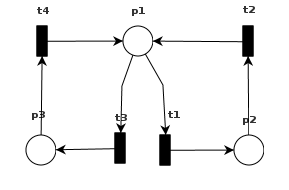
\includegraphics[height=5cm]{img/processo_seq_concorrenza.png}}
\caption{Processo sequenziale che presenta concorrenza sul posto p1}\label{fig:processo_seq_concorrenza.png}
\end{figure}

\begin{verbatim}PetriNet net;
Place net{p1,p2,p3};
Transition net{t1,t2,t3,t4};

// Modellazione flussi
net{ p1 -> t1 -> p2 -> t2 -> p1 | p1 -> t3 -> p3 -> t4 -> p1};

net::to_pnml_pipe("~/reti/processo_seq_concorrenza.xml");
\end{verbatim}

Il risultato della compilazione di tale codice è mostrato nella fugura \ref{fig:processo_seq_concorrenza.png}\footnote{Il file è stato modificato con il software pipe per poter avere un layout corretto}.

\section{Processi concorrenti su di una risorsa}
In questo esempio si modellano due processi con lo stesso comportamento e li si combina con un processo che descrive una generica risorsa che può essere libera oppure occupata. Il risultato è mostrato in figura \ref{fig:processi_concorrenti_su_risorsa.png}.
\begin{figure}[htb]
\centerline{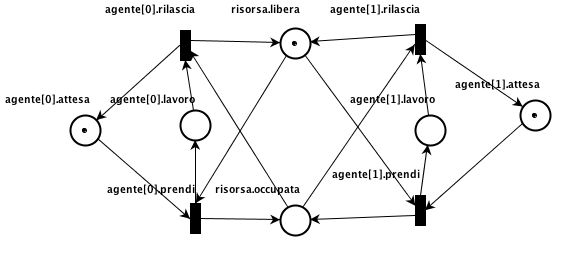
\includegraphics[height=5.5cm]{img/processi_concorrenti_su_risorsa.png}}
\caption{Rete che descrive due processi che concorrono per l'utilizzo di una risorsa}\label{fig:processi_concorrenti_su_risorsa.png}
\end{figure}

\begin{verbatim}PetriNet agente[2], risorsa;
Place agente{attesa, lavoro}, risorsa{libera, occupata};
Transition agente{prendi, rilascia}, risorsa{prendi, rilascia};

agente{attesa -> prendi -> lavoro -> rilascia -> attesa};
risorsa{libera -> prendi -> occupata -> rilascia -> libera};

agente{attesa=1};
risorsa{libera=1};

#union_add_prefix=True;
for(i=0;i<2;i+=1){
  agente[i] = (agente[i] | risorsa) on 
     [rilascia = rilascia as agente[i].rilascia, 
      prendi = prendi as agente[i].prendi];
 }
#union_add_prefix=False;
sys = (agente[0] | agente[1]) on [];

sys::to_pnml_pipe("~/Desktop/conc.xml");
\end{verbatim}

\section{Comunicazione tra due processi}
In questo classico esempio verrà modellato un sistema che simula l'azione di due processi {\tt sender} e {\tt receiver}.\\
Il processo {\tt sender} produrrà un messaggio, poi lo depositerà all'interno di un buffer e attenderà di ricevere un ack per poi rieffettuare lo stesso ciclo.\\
Il processo {\tt receiver} attenderà di ricevere un messaggio, invierà l'ack e consumerà il messaggio per poi effettuare lo stesso ciclo.\\

\begin{figure}[htb]
\centerline{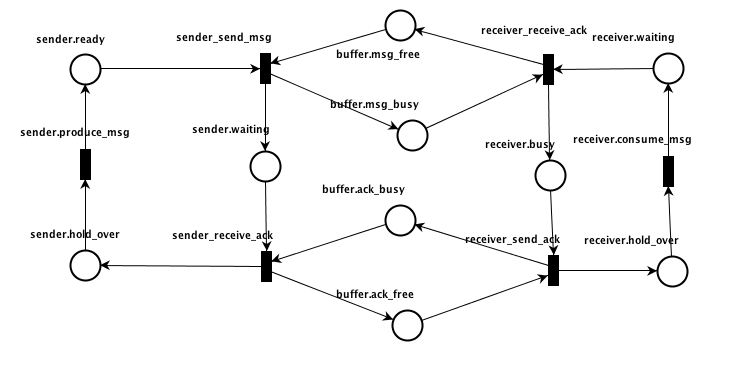
\includegraphics[width=12cm, height=8cm]{img/send_rec.png}}
\caption{Classico esempio di modellazione di un canale di comunicazione}\label{fig:send_rec.png}
\end{figure}

\begin{verbatim}PetriNet sender, receiver, buffer;
Place sender{ready, waiting, hold_over}, 
      receiver{waiting, busy, hold_over};
Place buffer{msg_free, msg_busy, ack_free, ack_busy};

Transition sender{produce_msg, send_msg, receive_ack}, 
           receiver{receive_msg, send_ack, consume_msg};
Transition buffer{push_msg, pop_msg, push_ack, pop_ack};

// Modellazione processo sender
sender{hold_over -> produce_msg -> ready -> 
       send_msg -> waiting -> receive_ack -> 
       hold_over};
// Modellazione processo receiver
receiver{waiting -> receive_msg -> busy -> 
         send_ack -> hold_over -> consume_msg ->
         waiting};
// Modellazione buffer
buffer{msg_free -> push_msg -> msg_busy -> pop_msg -> 
       msg_free | ack_free -> push_ack -> ack_busy -> 
       pop_ack -> ack_free};

#union_add_prefix = True;
s = (sender | receiver | buffer) on [send_msg = null = 
         push_msg as sender_send_msg, 
         receive_ack = null = pop_ack as sender_receive_ack, 
         null = send_ack = push_ack as receiver_send_ack,  
         null = receive_msg = pop_msg as receiver_receive_ack];

s::to_pnml_pipe("~/Desktop/send_rec.xml");

\end{verbatim}

Il risultato della compilazione di tale codice è mostrato nell'immagine \ref{fig:send_rec.png}.

\section{Problema lettori/scrittori}
Il seguente esempio mostra come modellare la rete che descrive il problema dei lettori e scrittori. L'esempio rispecchia quanto svolto da Tadao Murata in \cite{MURATA}.

\begin{figure}[htb]
\centerline{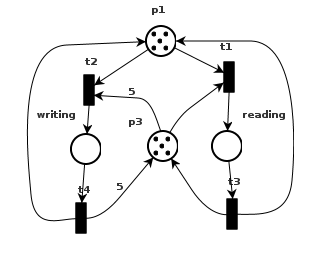
\includegraphics[width=7cm]{img/murata_writers_readers.png}}
\caption{Modellazione del problema lettori/scrittori}\label{fig:let_scrit.png}
\end{figure}

\begin{verbatim}PetriNet net;
Place net{reading(5), writing, p1(5), p3(5)};
Transition net{t1, t2, t3, t4};

net{p3 -> t1 -> reading -> t3 -> p3 
   | p3 ->(5) t2 -> writing -> t4 ->(5) p3};
net{p1 -> t1 | p1 -> t2 | t3 -> p1 | t4 -> p1};

net{p1=5, p3=5};

net::to_pnml_pipe("~/reti/murata_writers_readers.xml");
\end{verbatim}

Nalla figura \ref{fig:let_scrit.png} si può vedere il peso degli archi è stampato a video mentre non si vede la capacità dei posti. Con il software pipe è possibile verificare che la capacità viene inserita correttamente all'interno del file {\tt pnml}.

\section{I cinque filosofi}
Il seguente esempio mostra come si può modellare il classico problema
dei cinque filosofi proposto da Edsger Dijkstra nel 1965. Si può
notare come nell'ultima unione di reti si formi un conflitto sulle
forchette in quanto ogni filosofo modella già al suo interno la
presenza delle risorse e che quindi il parser fornisca qualche
avvertimento durante l'esecuzione del codice. Ciò però è ininfluente
ai fini del risultato in quanto gli archi necessari vengono inseriti
correttamente nella rete risultante.

\begin{figure}[htb]
\centerline{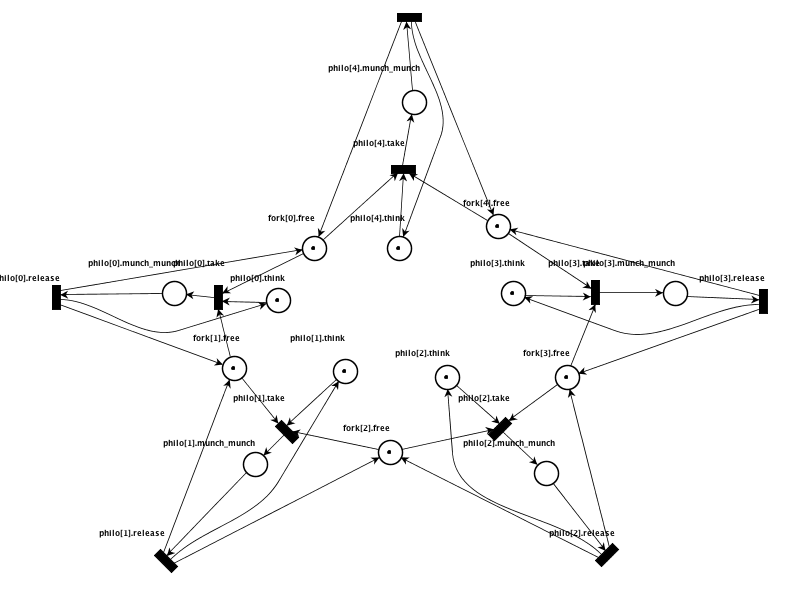
\includegraphics[width=12cm]{img/philosophers.png}}
\caption{Modellazione del problema lettori/scrittori}\label{fig:philosophers.png}
\end{figure}

\begin{verbatim}PetriNet philo[5], fork[5];
Place philo{munch_munch, think}, fork{free};
Transition philo{take, release}, fork{get, release};

philo{think=1};
fork{free=1};

philo{think -> take -> munch_munch -> release -> think};
fork{free -> get | release -> free};

#union_add_prefix=True;
for(i=0;i<5;i+=1){
philo[i] = (philo[i] | fork[i] | fork[i+1 % 5] ) on 
        [take = get = get as philo[i].take, 
         release = release = release as 
            philo[i].release ];
 }
#union_add_prefix=False;
sys = (philo[0] | philo[1] | philo[2] 
     | philo[3] | philo[4]) on [ ];
sys::to_dot("~/Desktop/philo", "png");
sys::to_pnml_pipe("~/Desktop/philo.pnml");
\end{verbatim}

\section{Rete con contatore di cicli}
Il seguente semplice esempio serve a mostare come gestire i posti di
capacità illimitata. In questo caso un posto viene utilizzato come
contatore dei cicli eseguiti dal sistema.

\begin{verbatim}PetriNet net;
Place net{istr1, istr2};
Transition net{t1, t2};
#default_place_capacity=unlimited;
Place net{contatore};
net{istr1 = 1};
net{istr1 -> t1 -> contatore | istr1 -> t1 -> istr2 -> t2 -> istr1};

net::to_pnml_pipe("~/Desktop/cont.pnml");

\end{verbatim}

%
\bibliography{bibliografia}
\bibliographystyle{alpha}
\end{document}
